\documentclass[11pt]{article}
\usepackage[utf8]{inputenc}
\usepackage[T1]{fontenc}
\usepackage{geometry}
\geometry{a4paper, margin=1in}
\usepackage{graphicx}
\usepackage{booktabs}
\usepackage{tabularx}
\usepackage{array}
\usepackage{float}
\usepackage{placeins}
\usepackage{changepage}
\usepackage{caption}
\captionsetup[figure]{font={footnotesize,it}, labelfont={footnotesize,it}, labelsep=period, justification=raggedright, singlelinecheck=false}
\captionsetup[table]{labelformat=empty, font=small, justification=raggedright, singlelinecheck=false}
\setlength{\parskip}{0.40em}
\setlength{\abovedisplayskip}{6pt plus 2pt minus 2pt}
\setlength{\belowdisplayskip}{6pt plus 2pt minus 2pt}
\setlength{\parindent}{0pt}
\setlength{\textfloatsep}{10pt plus 2pt minus 2pt}
\setlength{\intextsep}{10pt plus 2pt minus 2pt}
\renewcommand{\textfraction}{0.06}
\renewcommand{\topfraction}{0.92}
\renewcommand{\bottomfraction}{0.92}
\renewcommand{\floatpagefraction}{0.80}
\usepackage{hyperref}
\urlstyle{same}

\title{Report for the Course on Cyber-Physical Systems and IoT Security}
\author{Emilio Risi (matricola 2122841)}
\date{}

\begin{document}
\maketitle

\section*{Title of the reference paper}
Tractor Beam: Safe-hijacking of Consumer Drones with Adaptive GPS Spoofing (Noh, Kwon, Son, Shin, Kim, Choi, and Kim, ACM Transactions on Privacy and Security, Vol. 22, No. 2, Article 12, 2019)

\section*{Objectives}
The reference paper (Tractor Beam, Noh et al. 2019) shows that consumer autopilot drones (DJI Phantom 3/4, Parrot Bebop 2, 3DR Solo – all ArduPilot-based or proprietary) can be “safe-hijacked”: an adaptive GPS spoof that mimics the closing rate their return-to-home logic expects redirects the drone off course without tripping its EKF-based failsafe.

Our objective was to test whether this vulnerability generalizes to Betaflight, the dominant open-source firmware for low-cost hobbyist multirotors, whose “GPS Rescue” is the analog of the paper's return-to-home. Beyond adapting the attack, we extended it in two directions: (1) attempting to make the drone actually land at an attacker-chosen false home by decoupling Betaflight's position estimator from the spoofed GPS, and (2) simulating the RF power layer and training a discrete Soft Actor-Critic (soft Q-learning) agent to learn when to jam versus spoof.

\section*{System Setup}

\subsection*{Hardware-in-the-Loop (HITL) Attempt}
An early Hardware-in-the-Loop (HITL) setup was attempted using an FTDI adapter to simulate a GPS over UART. However, this was abandoned because injecting via UART primarily tests interface-level spoofing rather than the drone's internal state-estimation algorithms. Truly jamming and spoofing a physical GPS receiver would require prohibitively expensive RF hardware. Consequently, to precisely isolate and test how the firmware's rescue logic performs under attack, we chose a purely Software-in-the-Loop (SITL) environment.
\begin{figure}[H]
\centering
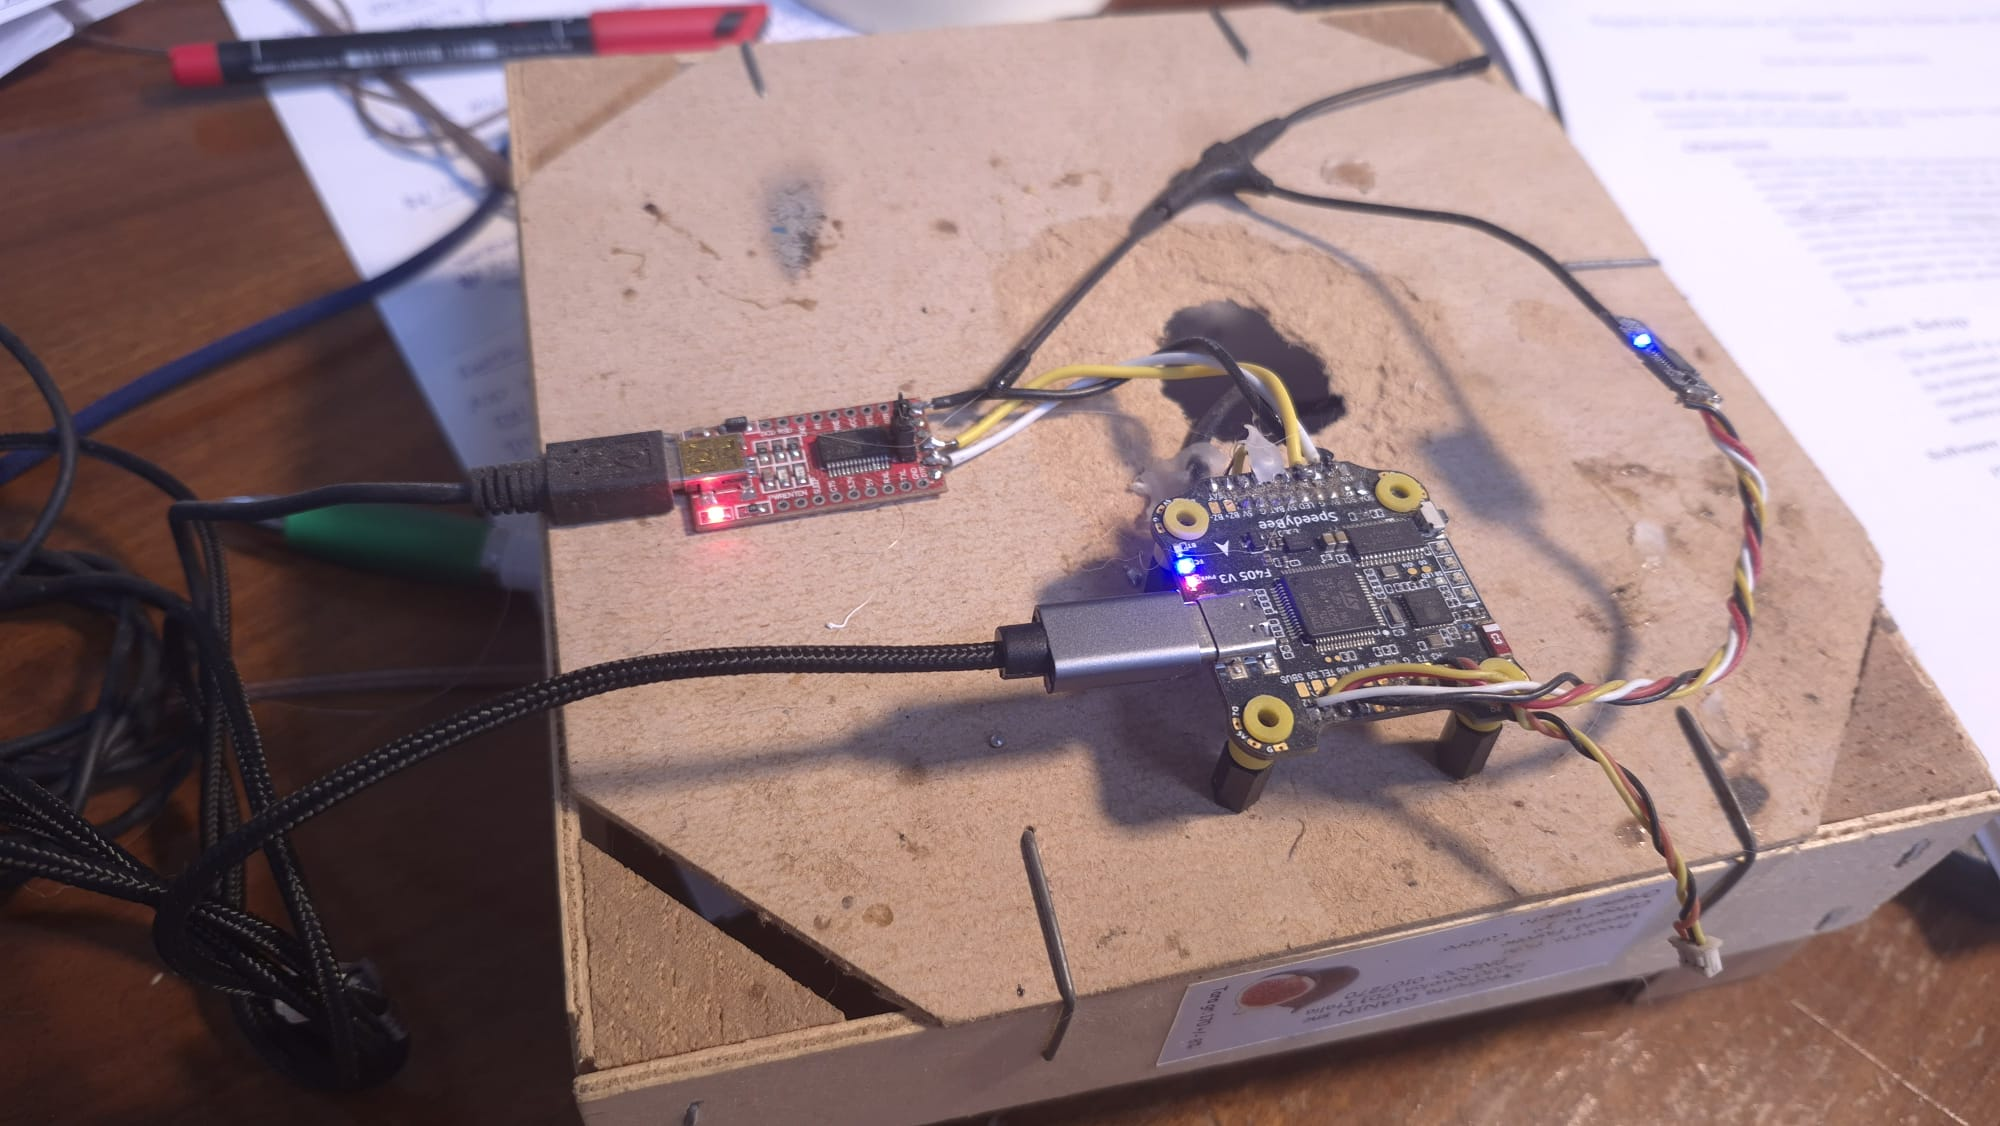
\includegraphics[width=0.7\textwidth]{figures/hitl_attempt.jpg}
\caption{Early HITL attempt using an FTDI adapter to simulate GPS over UART.}
\end{figure}

\subsection*{Tools Used}
The final investigation uses no physical hardware or RF transmission. Every sensor value the firmware sees is authored directly by our scripts, relying on two primary tools:

\begin{adjustwidth}{0.4in}{0in}
\noindent
\begin{minipage}[t]{0.13\textwidth}
  \vspace{0pt}
  
\includegraphics[width=0.75in,keepaspectratio]{logos/betaflight.png}
\end{minipage}%
\begin{minipage}[t]{0.87\textwidth}
  \vspace{0pt}
  \textbf{Betaflight.} Target firmware (v4.5), compiled to a native x86\_\allowbreak{}64 SITL (Software-In-The-Loop) binary with -DENABLE\_\allowbreak{}RESCUE\_\allowbreak{}PLAN=0 to exercise the classic GPS Rescue sanity-check controller (the newer default autopilot is out of scope).
\end{minipage}
\vspace{0.5em}

\noindent
\begin{minipage}[t]{0.13\textwidth}
  \vspace{0pt}
  
\includegraphics[width=0.75in,keepaspectratio]{logos/python.png}
\end{minipage}%
\begin{minipage}[t]{0.87\textwidth}
  \vspace{0pt}
  \textbf{Python 3.} Drives the whole simulation, attack, and analysis pipeline, speaking SITL's native UDP/TCP protocols directly (standard-library sockets, no MAVLink binding). NumPy carries the numerics (RF path-loss model, pure-Q-table SAC agent); Matplotlib renders the figures.
\end{minipage}
\vspace{0.5em}

\end{adjustwidth}

\subsection*{Betaflight vs. ArduPilot: Architecture and Flight Modes}
The two firmwares approach state estimation very differently, and that gap is the whole story. \textbf{ArduPilot} — the stack targeted in the original TractorBeam paper — is a mature autonomous navigation system built around an Extended Kalman Filter (EKF) that continuously cross-checks GPS against the IMU for statistical consistency.

\textbf{Betaflight} began as firmware for manual FPV racing (modes like \textbf{ACRO} and \textbf{ANGLE}) and only recently bolted on autonomous-style features — most notably \textbf{GPS Rescue} (Return-to-Home) — to support long-range flight. It does run a primitive estimator — independent 1-D Kalman filters for position — but, unlike ArduPilot's coupled EKF, the rescue logic never consults their trust or variance: it simply points at the recorded home, pitches forward, and watches basic \textbf{rate-of-change sanity checks}. That makes it uniquely susceptible to an attacker who injects fake sensor data matching the expected rate of progress — the same weakness now shipping on far cheaper, far more numerous airframes. (We contrast the two detectors in detail in the Integrated Scenario and Comparison with the Original Attack section.)

Attitude is estimated just as cheaply. Where ArduPilot's EKF fuses every sensor into a single statistically-weighted state, Betaflight tracks orientation with a \textbf{Mahony/DCM complementary filter}: it integrates the gyroscope for fast, short-term rotation and continuously nudges that estimate back toward the "down" direction the accelerometer reports (i.e. gravity), a lightweight alternative to full statistical fusion. The filter carries no notion of trust or innovation variance, but it does constantly cross-check the drone's attitude against the accelerometer — and that single cross-check, as we show below, turns out to be the one obstacle a GPS-only spoof cannot get past.

\begin{figure}[H]
\centering
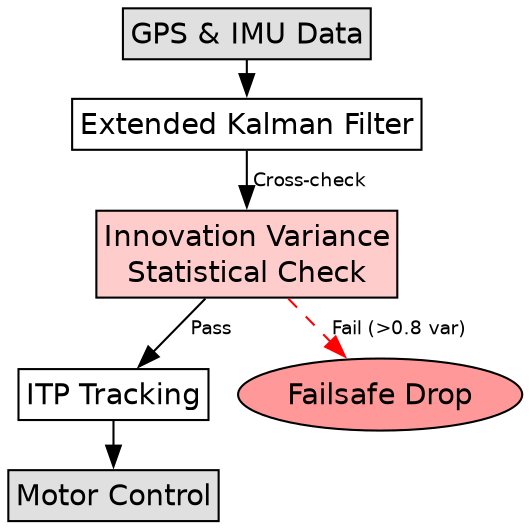
\includegraphics[width=0.45\textwidth]{figures/ardupilot_arch.png} \hfill
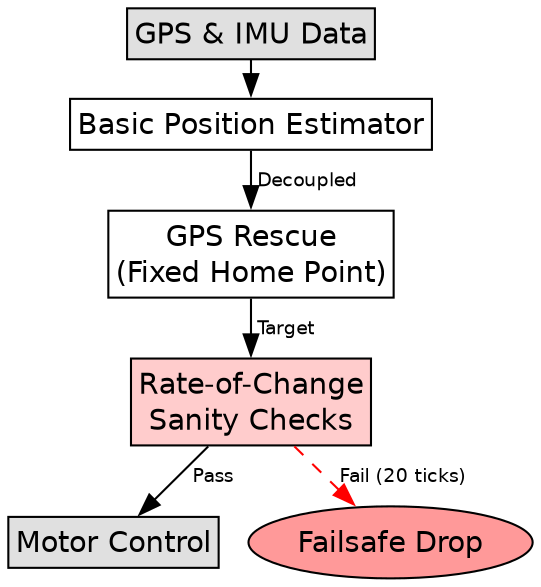
\includegraphics[width=0.45\textwidth]{figures/betaflight_arch.png}
\caption{Architectural differences between ArduPilot (left) and Betaflight (right).}
\end{figure}

\subsection*{SITL Simulation Environment}
The exact Betaflight firmware (C) is compiled as a native x86 SITL binary, completely isolated from real hardware. It receives all sensor inputs over the network — our Python harness is the sole source of every GPS, IMU, and RC value the firmware ever sees.
\begin{figure}[H]
\centering
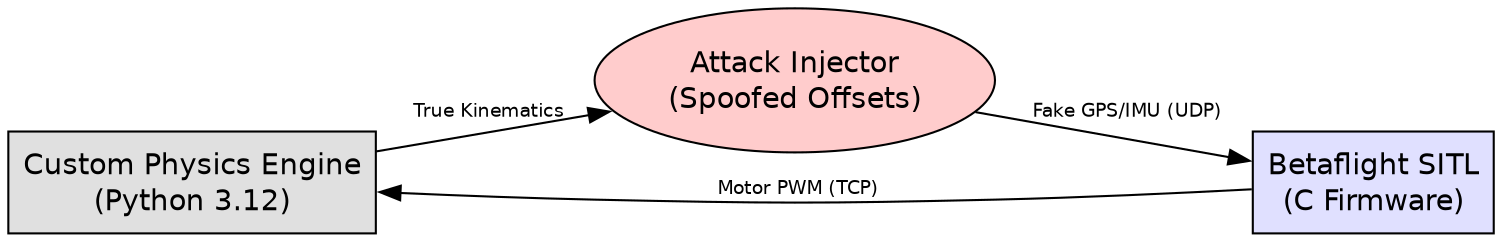
\includegraphics[width=0.8\textwidth, height=2.2in, keepaspectratio]{figures/sitl_arch.png}
\caption{SITL simulation loop closing the physics engine with Betaflight over UDP/TCP.}
\end{figure}

\subsection*{Python Harness}
The harness authors the full physics state each tick and closes the loop with the firmware over three sockets. The \textbf{state channel} streams a fabricated flight-dynamics packet over UDP — position, ENU velocity, an orientation quaternion, angular rates and linear acceleration — carrying everything the firmware would otherwise read from its GPS and IMU. A second \textbf{UDP channel} injects the sixteen RC channels (arming and flight-mode switches) that a pilot's radio would supply. Finally, an \textbf{MSP link} over TCP reads the firmware's own state back — the GPS-Rescue phase, failure code and distance-to-home, plus the armed flag — which the harness uses to decide whether each spoof was accepted or rejected.

\textbf{Kinematics we author directly:}
\par\hangindent=1.8em\hangafter=1\hspace*{1.2em}$\bullet$ \textbf{Attitude:} Betaflight's SITL applies a fixed conjugation to the quaternion we send, which we invert so the firmware reads the pitch $\theta$ we intend: $q = \left(k\cos(\theta/2),\ k\sin(\theta/2),\ -k\sin(\theta/2),\ k\cos(\theta/2)\right)$, $k=\sqrt{0.5}$.
\par\hangindent=1.8em\hangafter=1\hspace*{1.2em}$\bullet$ \textbf{Accelerometer consistency:} the attitude filter overrides the injected quaternion within one cycle from the accelerometer, so we supply the matching body-frame vector from the rotation matrix's earth-up row, $a = \left(g\sin\theta,\ 0,\ -g\cos\theta\right)$.
\par\hangindent=1.8em\hangafter=1\hspace*{1.2em}$\bullet$ \textbf{Velocity and heading:} GPS-heading confidence needs a velocity consistent with the pitched attitude, so we convert bearing $\beta$ and speed $v$ to ENU: $v_E = v\sin\beta$, $v_N = v\cos\beta$.
\par\hangindent=1.8em\hangafter=1\hspace*{1.2em}$\bullet$ \textbf{Coordinate mirroring:} SITL mirrors lat/lon about an origin latched from the first packet, $\mathrm{send} = 2\,\mathrm{origin} - \mathrm{desired}$; the packet builder pre-mirrors so callers set the position they want the firmware to see.
\par\hangindent=1.8em\hangafter=1\hspace*{1.2em}$\bullet$ \textbf{RF layer:} free-space path loss at GPS L1 ($1575.42$ MHz), $\mathrm{FSPL} = 20\log_{10} d + 20\log_{10} f - 27.55$ dB, sets the received power that classifies the regime (normal / spoofed / jammed).


\section*{Experiments}

\subsection*{Sanity Checks and Attack Design}
We reframed the paper's mechanism as a directly testable question per sensor channel: given a spoofed sensor feed, does the firmware follow it (accept) or trigger a fail-safe (reject)? Betaflight's GPS Rescue exposes exactly this kind of check on two independent channels, both structurally identical – a per-tick progress-rate ratio against an internally computed target, accumulated over a fixed failing window:
\begin{figure}[H]
\centering
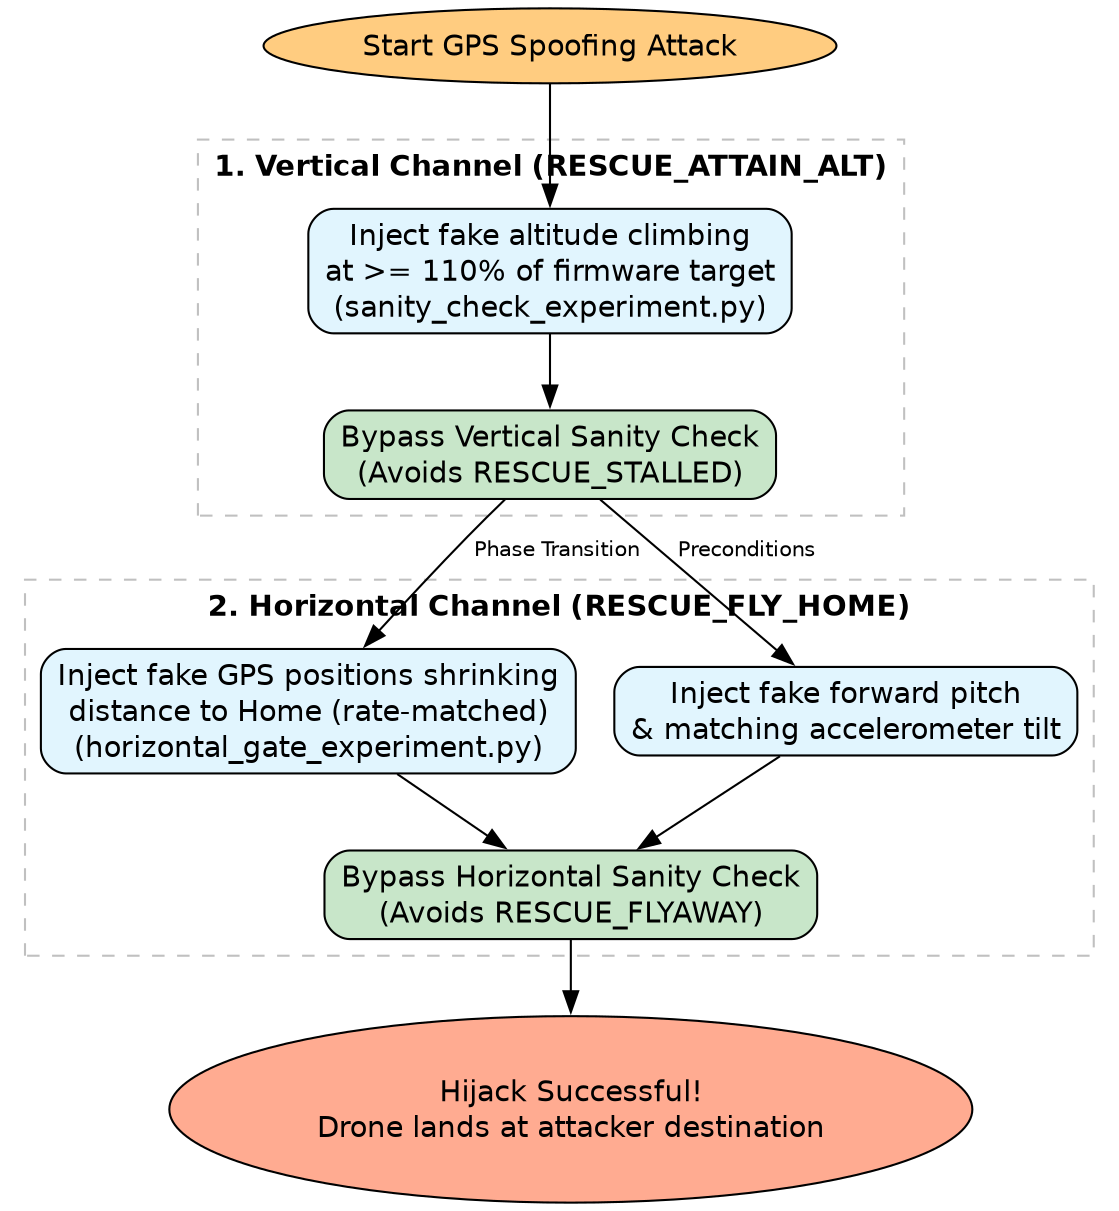
\includegraphics[width=0.85\textwidth, height=4.0in, keepaspectratio]{figures/attack_flow.png}
\caption{Flowchart of the two-stage spoofing attack to bypass Betaflight GPS Rescue sanity checks.}
\end{figure}

\subsubsection*{Locating the Sanity Check in Betaflight's Source}
The paper describes the vulnerability only in the abstract — a check that tests the \textbf{plausibility} of the drone's movement, not its ground truth. To make it concrete we traced that check into Betaflight's flight code (gps\_\allowbreak{}rescue\_\allowbreak{}multirotor.c) and found that both channels reduce to the \textbf{same leaky-counter rule}, evaluated once per second. Writing c for the failing counter, r for the channel's progress ratio (the measured rate divided by the firmware's own target rate for that tick), $\tau$ for the acceptance threshold and N for the trip count:
\[
c_{k+1} = \max\!\left(0,\; c_k + \delta_k\right), \qquad
\delta_k = +1 \ \mbox{if}\ r_k < \tau, \quad \delta_k = -1 \ \mbox{otherwise}; \qquad
c_k \ge N \ \Rightarrow \ \mbox{fail-safe}.
\]
The counter is a bounded random walk: it climbs by one on every tick that falls short of the target rate and \textbf{leaks} by one (never below zero) on every tick that meets it, so the fail-safe fires only after a net N shortfalls accumulate. The consequence is the whole vulnerability in one sentence: an attacker never has to win every tick, only keep more ticks above $\tau$ than below it. A spoofed feed whose reported progress sits above the threshold \textbf{on average} therefore never trips the check — which is exactly why an adaptive, rate-matched spoof gets through. The two channels differ only in which quantity plays the role of r, and in ($\tau$, N):
\begin{itemize}
\item \textbf{RESCUE\_\allowbreak{}ATTAIN\_\allowbreak{}ALT} (the vertical/altitude gate): r = (measured altitude change) $\div$ (the firmware's own target climb for that tick), $\tau$ = 0.5, N = 10. Ten net ticks of climbing at less than half the commanded rate raise \textbf{RESCUE\_\allowbreak{}STALLED}.
\item \textbf{RESCUE\_\allowbreak{}FLYAWAY} (the horizontal gate): r = (closing speed toward home) $\div$ (target ground speed), $\tau$ = 0.2, N = 20. It is the identical counter applied to horizontal progress, but it is only \textbf{live} once the rescue reaches its \textbf{RESCUE\_\allowbreak{}FLY\_\allowbreak{}HOME} phase — four phases after the trigger — which is what forces the ordering discussed below.
\end{itemize}

With the rule pinned down, each test profile is simply a deliberately chosen value of the progress ratio r, sweeping from clearly-rejected to clearly-accepted so we can locate the acceptance boundary:

\textbf{1. Vertical profiles} (sanity\_\allowbreak{}check\_\allowbreak{}experiment.py) — expressed as a fraction of the firmware's own ascend rate, i.e. of the $\tau$ = 0.5 gate:
\par\hangindent=1.8em\hangafter=1\hspace*{1.2em}$\bullet$  \textbf{static (0\%)} — no climb at all; a floor control that must be rejected.
\par\hangindent=1.8em\hangafter=1\hspace*{1.2em}$\bullet$  \textbf{slow (8\%)} and \textbf{partial (30\%)} — climbing, but below the half-rate threshold: slow should always fail, while partial sits just under the boundary to probe it.
\par\hangindent=1.8em\hangafter=1\hspace*{1.2em}$\bullet$  \textbf{adaptive (110\%)} — meets and slightly exceeds the commanded climb (r > $\tau$); the rate-matched feed that should pass.

\textbf{2. Horizontal profiles} (horizontal\_\allowbreak{}gate\_\allowbreak{}experiment.py):
\par\hangindent=1.8em\hangafter=1\hspace*{1.2em}$\bullet$  \textbf{frozen (no progress)} and \textbf{naive-jump (instant teleport to home)} — the two crude spoofs a naive attacker would try; both report an implausible closing speed and are rejected controls.
\par\hangindent=1.8em\hangafter=1\hspace*{1.2em}$\bullet$  \textbf{adaptive-home} — a rate-matched convergence on the \textbf{true} home at the target ground speed: the honest-looking trajectory the gate is meant to accept.
\par\hangindent=1.8em\hangafter=1\hspace*{1.2em}$\bullet$  \textbf{adaptive-fake-destination} — the same rate-matched convergence, but aimed at an attacker-chosen point 150 m off the true home; this is the actual hijack, testing whether the gate will follow an attacker's trajectory just as readily as the real one.

We had to clear the two channels strictly in order, and not by choice. The checks live in different phases of one state machine that the drone always traverses in sequence — RESCUE\_\allowbreak{}ATTAIN\_\allowbreak{}ALT $\rightarrow$ RESCUE\_\allowbreak{}PITCH\_\allowbreak{}FORWARD $\rightarrow$ RESCUE\_\allowbreak{}ROTATE $\rightarrow$ RESCUE\_\allowbreak{}FLY\_\allowbreak{}HOME — and the horizontal gate is only evaluated in FLY\_\allowbreak{}HOME, four phases past the altitude gate. The drone therefore never even reaches the horizontal check until the vertical one has been satisfied. Clearing the altitude gate, in turn, demanded more than fake GPS coordinates: Betaflight only advances the rescue when it is fed a mathematically consistent combination of forward pitch, a matching accelerometer tilt, and a matching horizontal velocity. If the accelerometer disagrees with the pitch, the Mahony/DCM attitude filter introduced earlier overrides the injected orientation within about one filter cycle and the rescue stalls — so the vertical channel is really a joint attitude-and-altitude gate that has to be defeated first.

Finally, because some profiles yielded inconsistent results across full-suite re-runs, we ran statistical repeats (up to six times each) on a fresh simulated drone to characterise the outcome distributions. These profiles are part of a larger reproduction requiring $\sim$55 firmware-in-the-loop SITL runs. The total wall-clock cost is $\sim$55 minutes on an Intel Core i5 (16GB RAM) laptop, as each run boots a fresh Betaflight process and flies a full rescue in real time to avoid injecting timing jitter into the bimodal outcomes. A full runtime breakdown is provided in Appendix C, and the per-profile outcome summary is tabulated in Appendix B.
\begin{figure}[H]
\centering
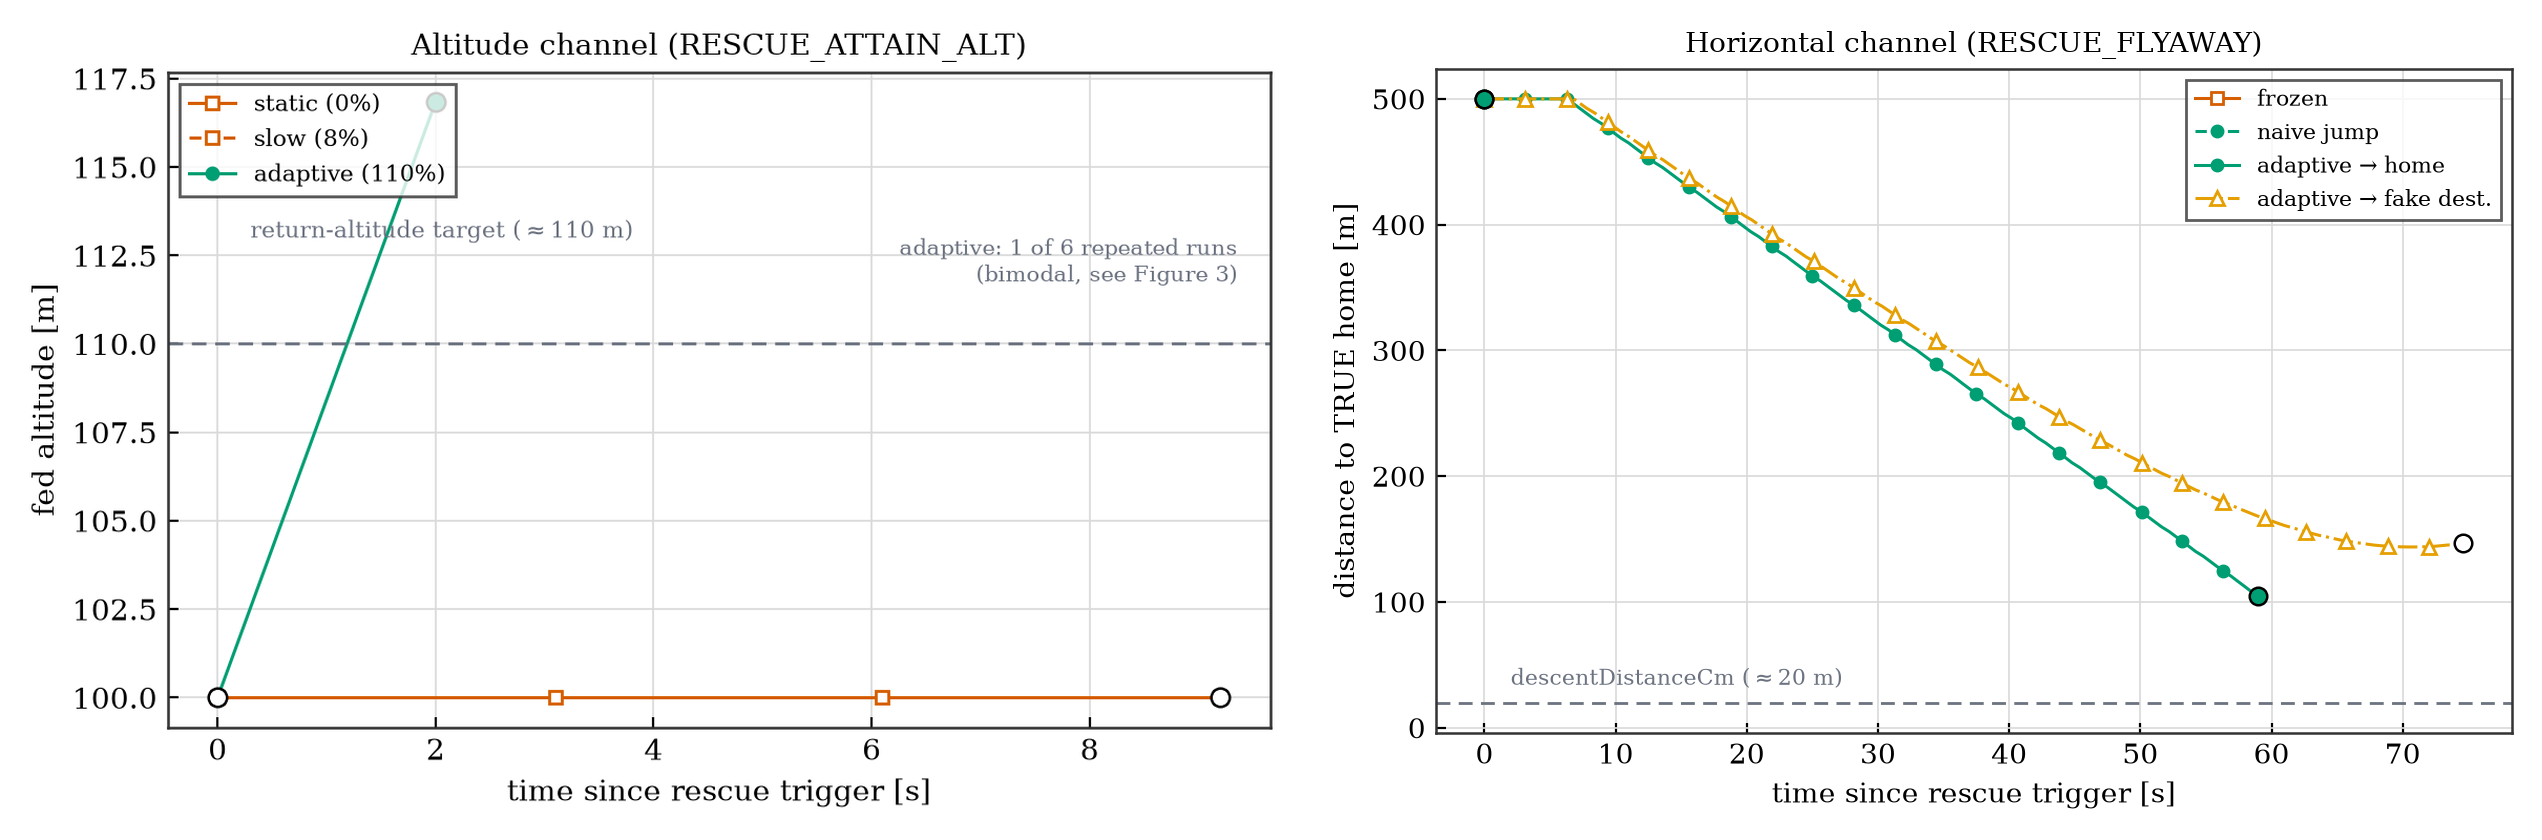
\includegraphics[width=0.9\textwidth, height=2.9in, keepaspectratio]{figures/fig1_2_combined.png}
\caption{Sanity checks. Left: Altitude channel (fed altitude vs. time). Right: Horizontal channel (distance to true home vs. time).}
\end{figure}

\subsection*{Estimator Decoupling (False Home)}
To go beyond redirecting and actually land at a false home, we attacked the position estimator itself. Betaflight computes distance-to-home from the Kalman-filtered position estimate (position\_\allowbreak{}estimator.c), anchored to the armed-at home; the landing gate is distance-to-home < 20 m. We froze the spoofed GPS at a false home B = 150 m north of the true home and fed a velocity toward the true home, decoupling the estimator from the GPS. Sweeping the velocity reveals how far the estimate can be dragged before the rescue rejects it.

\subsection*{Attack Execution Algorithms}
With the sanity checks characterised, we can assemble them into a complete attack. We formalise two variants that pursue the same physical goal — jam the link to force GPS Rescue, then rate-match a spoof past the gates — but differ in how they choose transmit power: a \textbf{deterministic} attack that computes the power from a closed-form path-loss model, and a \textbf{reinforcement-learning} attack that learns it. Both operate over the same RF layer: a free-space path-loss model of the GPS L1 link (1575.42 MHz, src/tractorbeam/rf\_\allowbreak{}sim.py) that maps the attacker's transmit power and range to the regime the receiver ends up in — normal, spoofed, or jammed.

\subsubsection*{Algorithm 1: Deterministic Attack Strategy}
The deterministic attack fixes the power schedule ahead of time. Knowing the geometry, the attacker computes from free-space path loss exactly how much power jams the genuine signal, and how much then holds the spoof just above the authentic-signal margin, and executes a fixed sequence:
\begin{enumerate}
\item \textbf{Setup \& tracking:} the attacker passively tracks the drone via its 5.8 GHz analog video feed, a signal GPS jamming does not touch.
\item \textbf{Failsafe trigger (jamming):} broadcast GPS L1 noise at maximum power to deny the authentic signal, forcing Betaflight into GPS Rescue.
\item \textbf{Estimator decoupling (spoofing):} once Rescue is active, switch to spoofing and drop transmit power to +3 dB above the theoretical authentic signal (from the free-space path-loss formula), so the receiver locks onto the spoof without saturating.
\item \textbf{Kinematic rate-matching:} feed synthetic, rate-matched altitude and velocity so the altitude and flyaway counters never trip — the r > $\tau$ condition of the previous section.
\item \textbf{Hijack completion:} the internal estimator decouples and its perceived position drags toward the attacker, reaching the target location. A perfect exploit would cross the < 20 m ring for a gentle landing; instead, Betaflight's altitude gate interrupts the rescue and forces a fail-safe descent at the attacker's location.
\end{enumerate}

\subsubsection*{Algorithm 2: Reinforcement Learning (discrete SAC) Strategy}
The reinforcement-learning variant replaces that hand-computed schedule with a learned one — useful when the geometry is not known in advance. We cast the power decision as a Markov Decision Process over the same RF layer and train a \textbf{discrete Soft Actor-Critic (soft Q-learning)} agent: a tabular, maximum-entropy Q-learner in NumPy (experiments/rl\_\allowbreak{}jam\_\allowbreak{}spoof.py), which suffices for this low-dimensional problem and needs no deep network. Its state is the attack goal (hijack vs. disrupt) and the drone's range; its action is a choice among discrete transmit-power levels (dBm). The received power is computed from path loss and used only to classify the regime for the reward, never observed directly. A large positive reward is paid for reaching a 'Lock' (spoof power > genuine + 3 dB) or 'Jam' (power > saturation), minus a penalty proportional to power that pushes the agent toward a stealthier footprint. The learned procedure mirrors Algorithm 1 step for step:
\begin{enumerate}
\item \textbf{Setup \& tracking:} identical to the deterministic approach; the agent observes only the attack goal and the drone's range.
\item \textbf{Adaptive failsafe trigger:} for the disrupt goal, the agent learns the power level that places the receiver in the jammed regime (above saturation), forcing GPS Rescue.
\item \textbf{Learned decoupling:} for the hijack goal, instead of a hardcoded formula, it learns the power level that lands the receiver in the spoofed regime — just above the capture margin — holding the estimator without saturating.
\item \textbf{Reward shaping:} a per-step penalty proportional to transmit power trades raw dominance for the minimum power that still achieves the regime, shrinking the RF footprint.
\item \textbf{Hijack completion:} the drone reaches the attacker's false home but is forced down via fail-safe due to the altitude gate; the agent converges on a working high-power schedule, though it fails to find the minimal stealth power (see Results). A different reinforcement learning approach should be implemented to better minimize it.
\end{enumerate}

\begin{figure}[H]
\centering
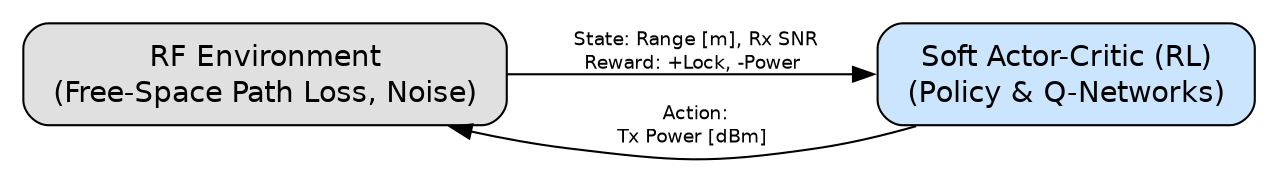
\includegraphics[width=0.65\textwidth]{figures/rl_arch.png}
\caption{Soft Actor-Critic agent environment.}
\end{figure}

\section*{Results and Discussion}

\subsection*{False Home Results}
\begin{table}[H]\centering\small
\caption{\textbf{False-home landing distribution over N=6 repeats per velocity (B = 150 m).}}
\begin{tabular}{lccc}
\toprule
\textbf{Spoofed velocity (B = 150 m)} & \textbf{Reached fly-home} & \textbf{Landed at false home} & \textbf{Max divergence (m)} \\
\midrule
7.5 m/s & 6/6 & 0/6 & 16\\
30 m/s & 3/6 & 0/6 & 62\\
60 m/s & 5/6 & 0/6 & 126\\
65 m/s & 3/6 & 0/6 & 0\\
70 m/s & 2/6 & 0/6 & 0 \\
\bottomrule
\end{tabular}
\end{table}

Estimator decoupling (Figure 9, Appendix B; table above): with the spoofed GPS frozen at B = 150 m and a velocity fed toward true home, the Kalman estimate lags the frozen GPS. Two robust facts emerge from the N=6 repeats per velocity. First, when a run reaches the fly-home leg and decouples, the maximum estimate-vs-GPS divergence tracks a first-order lag of $\sim$2.1 s almost exactly — $\sim$16 m at 7.5 m/s, 62 m at 30 m/s, 126 m at 60 m/s (2.1$\cdot$v predicts 15.7, 63, 126 m), so the mechanism is real and quantitatively understood. Second, while the drone successfully reached the target location, a gentle landing at the false home never reproduced: 0 of 30 runs. We identified the altitude gate as the primary cause blocking a full landing — its per-run running-maximum target makes most runs stall and triggers a fail-safe descent before crossing the 20 m landing ring. The honest conclusion: decoupling is a genuine, measurable effect that redirects the drone to the attacker, but the nondeterministic altitude gate interrupts the rescue and forces a descent rather than a safe landing.

\subsection*{RF Layer and Reinforcement Learning Results}

\begin{table}[H]\centering\small
\caption{\textbf{RF layer training outcomes (discrete power states).}}
\begin{tabular}{lcccc}
\toprule
\textbf{Goal} & \textbf{Range} & \textbf{Learned P (dBm)} & \textbf{Deterministic P (dBm)} & \textbf{Regime} \\
\midrule
hijack & 75 m & -29.4 & -50.3 & spoofed\\
hijack & 150 m & -20.6 & -45.1 & spoofed\\
hijack & 300 m & -38.1 & -39.8 & spoofed\\
hijack & 600 m & -8.4 & -32.9 & spoofed\\
disrupt & 75 m & 28.3 & -24.1 & jammed\\
disrupt & 150 m & 23.0 & -18.9 & jammed\\
disrupt & 300 m & 16.0 & -11.9 & jammed\\
disrupt & 600 m & 9.0 & -6.7 & jammed \\
\bottomrule
\end{tabular}
\end{table}

\begin{table}[H]\centering\small
\caption{\textbf{Baseline reward comparison.}}
\begin{tabular}{lc}
\toprule
\textbf{Policy} & \textbf{Avg episode return} \\
\midrule
random & $\sim$6-7\\
naive fixed-power & $\sim$82\\
deterministic (analytic min) & $\sim$82-85\\
learned (RL) & $\sim$83-87 \\
\bottomrule
\end{tabular}
\end{table}

RF + RL (Figures 10-11, Appendix B): the learned policy chooses spoofing (medium power, capture window) for hijack and jamming (high power, saturation) for disruption - 'when to jam' emerges from the same discrete power action set. Average episode return: random $\sim$6-7, naive $\sim$82, deterministic (analytic minimum) $\sim$82-85, learned $\sim$83-87. The learned policy matches, but does not beat, the deterministic optimum: with a known deterministic plant the RL rediscovers the closed-form answer. It also learns the regime but not the minimal power, because the reward's power penalty is negligible versus the +100 success reward. Another RL approach should be implemented to better minimize the transmit power.

\subsection*{Integrated Scenario and Comparison with the Original Attack}
Figure 7 ties the three layers end to end — passive tracking, GPS L1 jamming to force Rescue, then adaptive spoofing with estimator decoupling. Unlike the SITL sweep above, this integrated timeline is a \textbf{deterministic end-to-end model} (attack\_\allowbreak{}scenario.py) with a simplified first-order estimator, used to visualise the full chain and to map our measurements onto the paper's quality metrics. Its numbers are a best-case illustration, not a claim that the firmware lands reliably; the reproducible SITL result is the bounded decoupling reported above.
\begin{figure}[H]
\centering
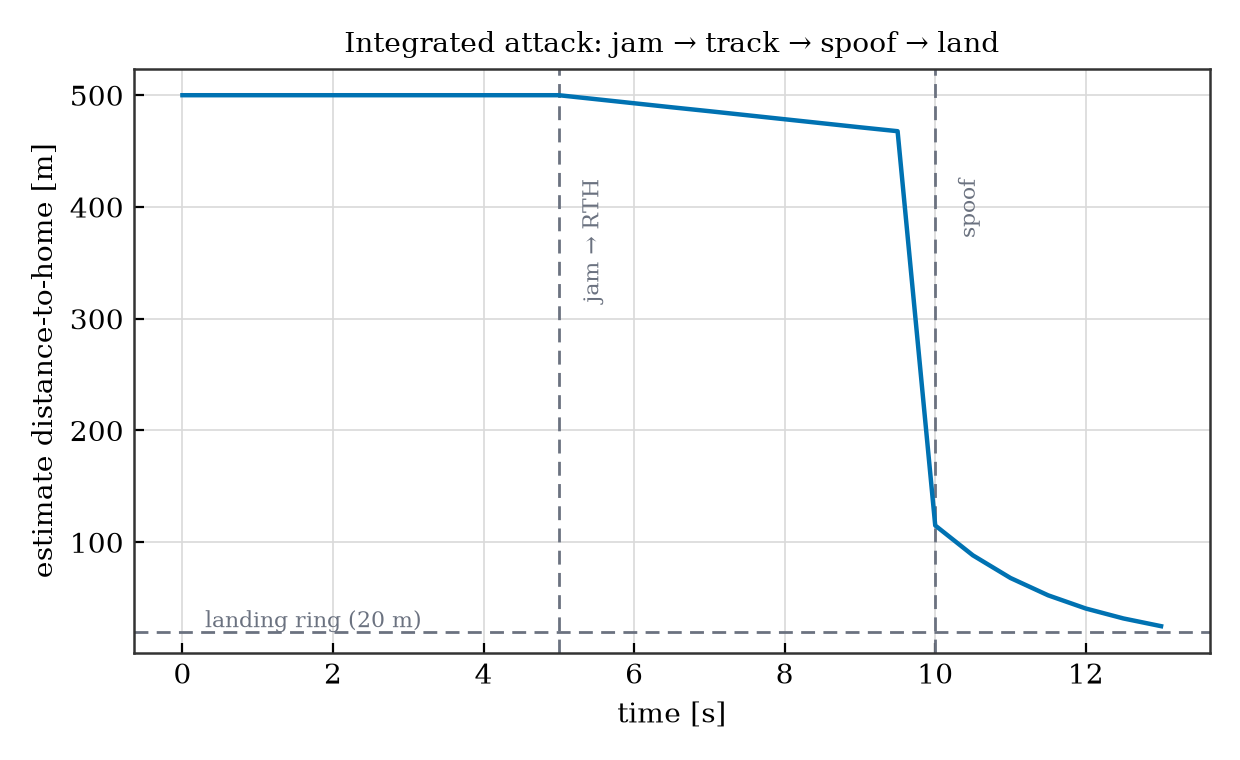
\includegraphics[width=0.6\textwidth]{figures/fig7_attack_scenario.png}
\caption{Overall timeline: passive tracking, GPS L1 jamming (forcing Rescue), followed by adaptive spoofing and estimator decoupling to false home.}
\end{figure}

\begin{table}[H]\centering\small
\caption{\textbf{Hijack quality metrics from the deterministic end-to-end model, mapped to the paper's.}}
\begin{tabular}{l>{\raggedright\arraybackslash}p{3in}}
\toprule
\textbf{Hijack quality metric (paper analog)} & \textbf{Value} \\
\midrule
Max divergence (EKF-innovation analog) & 130.3 m\\
Min FLYAWAY margin (leash analog) & 6.96\\
Landing bearing (safe-direction analog) & 90 deg\\
Landing error vs. attacker & 0 m\\
Time to land & 13.5 s \\
\bottomrule
\end{tabular}
\end{table}

The tracking layer is what makes this practical. The attacker sits on the drone's return path (150 m from home), jams the link to trigger RTH, and tracks the craft passively by direction-finding on its 5.8 GHz FPV video — a signal the GPS L1 jammer does not touch — then spoofs from that position until the firmware forces a fail-safe descent next to the attacker, rather than at its armed-at home. Tracking quality, not jammer power, bounds a believable spoof: a simple RSSI rig reaches only $\sim$60 m, a pseudo-Doppler array $\sim$220 m.

Four differences stand out from the original attack. \textbf{Detector:} ArduCopter uses an EKF innovation-variance test (squared velocity innovations, tripping when variance stays > 0.8 for $\sim$1 s); Betaflight's legacy GPS Rescue uses simple rate-ratio checks and never gates on estimator trust. \textbf{Estimator:} both run a Kalman filter, but Betaflight's position-trust (trustXY) is not wired into the rescue as a detector. \textbf{Path model:} the paper's drones track a moving intermediate target point with a leash length, whereas Betaflight flies straight at a single recorded home point. \textbf{Outcome (the main deviation):} the paper's safe-hijack ends in a gentle controlled landing at the attacker's spot; ours never perceives arriving home, so it comes down via the fail-safe — redirection plus a forced descent, with the RF power layer quantified separately, which the paper leaves implicit.

\subsection*{Overall Attack Efficacy}
In short, Tractor Beam's core claim generalises: Betaflight has no raw-GPS glitch detector anywhere, and both rescue gates are the same evadable rate-check, so the vulnerability is not specific to the paper's ArduPilot targets. Two things temper it. The attack needs \textbf{three consistent channels, not one} — spoofed GPS does nothing until a matching pitch and accelerometer tilt satisfy the separate Mahony/DCM attitude filter — and it is the \textbf{legacy} GPS Rescue controller, not the default build, that is vulnerable. Near the threshold the outcome is probabilistic (Figure 8, Appendix B), landing on one of two fixed values as the per-run altitude target varies.

\section*{Conclusion}
Testing this low-cost, open-source architecture against the paper's proprietary and ArduPilot platforms shows the vulnerability is not an artifact of expensive hardware: the core vulnerability generalizes (allowing redirection and forced descent), and the cheaper board reaches a far larger installed base. The differences that matter are architectural rather than economic – Betaflight's simpler rate-ratio detector is easier to evade with a cruder spoof, while its unused Kalman trust value is the one statistical signal that would catch the attack. Low cost buys no extra security here; it moves the same weaknesses onto cheaper, more widespread hardware.

A note on firmware version and scope. The controller exercised here is Betaflight's legacy GPS Rescue, selected at build time with -DENABLE\_\allowbreak{}RESCUE\_\allowbreak{}PLAN=0 — the historical rescue path and, today, the fallback on flash-constrained boards rather than the newest default. Current full-feature builds default instead to a newer flight-plan autopilot that flies the rescue as a waypoint mission, and this logic has continued to be hardened across releases. Our results therefore characterise the legacy controller — still widely deployed on cheaper and older hardware — and not the latest default; repeating these experiments against the current flight-plan autopilot, which exposes no equivalent debug telemetry yet, would be a worthwhile extension. We did not test it, but expect the attack's core to carry over: the real weakness is the position estimator, not the rescue controller, and the newer autopilot still consumes Betaflight's 1-D Kalman estimate — whose trust/variance is never gated on, with no raw-GPS glitch check anywhere. Unless the flight-plan code adds the innovation-variance gating Betaflight otherwise lacks, a rate-matched spoof should still mislead it; the extra mission staging may reject cruder spoofs, but more planning logic is not statistical trust.

\section*{References}
\begin{itemize}
    \item[ {[1]} ] Original TractorBeam Attack: \textit{TractorBeam: Hijacking Drones with Rate-Matched GPS Spoofing}. (Targeting ArduPilot EKF).
    \item[ {[2]} ] Betaflight Open Source Flight Controller: \url{https://github.com/betaflight/betaflight}.
    \item[ {[3]} ] Just Command Runner: \url{https://github.com/casey/just}.
\end{itemize}

\newpage
\appendix
\section*{Appendix A: Terminology and Script Dictionary}
\begin{table}[H]\centering\small
\caption{\textbf{Terminology and script dictionary.}}
\begin{tabular}{>{\raggedright\arraybackslash}p{2.0in}>{\raggedright\arraybackslash}p{1.0in}>{\raggedright\arraybackslash}p{2.8in}}
\toprule
\textbf{Term / Script} & \textbf{Type} & \textbf{Description} \\
\midrule
src/tractorbeam/sitl\_\allowbreak{}transport.py & Python Script & Custom UDP/TCP harness connecting Betaflight SITL to synthetic physics.\\
experiments/sanity\_\allowbreak{}check\_\allowbreak{}experiment.py & Python Script & Profiles the vertical GPS Rescue sanity checks.\\
experiments/horizontal\_\allowbreak{}gate\_\allowbreak{}experiment.py & Python Script & Profiles the horizontal GPS Rescue checks (flyaway).\\
experiments/false\_\allowbreak{}home\_\allowbreak{}landing.py & Python Script & Demonstrates estimator decoupling and forced landing at a false home.\\
src/tractorbeam/rf\_\allowbreak{}sim.py & Python Module & Free-space GPS L1 path-loss / regime model used by the RF experiments.\\
experiments/rl\_\allowbreak{}jam\_\allowbreak{}spoof.py & Python Script & Trains and evaluates the tabular soft-Q-learning (discrete SAC) jam/spoof agent.\\
B & Variable & False home distance (e.g., B = 150 m).\\
v & Variable & Spoofed horizontal velocity vector.\\
GPS L1 & Terminology & The primary GPS frequency band (1575.42 MHz) targeted by the spoofer.\\
discrete SAC & Terminology & Discrete Soft Actor-Critic (soft Q-learning): a tabular, maximum-entropy Q-learner over discrete power actions. \\
\bottomrule
\end{tabular}
\end{table}

\newpage
\section*{Appendix B: Supplemental Experimental Graphs}

\begin{table}[H]\centering\small
\caption{\textbf{Outcome summary across all eight profiles.}}
\begin{tabular}{>{\raggedright\arraybackslash}p{0.6in}>{\raggedright\arraybackslash}p{0.9in}>{\raggedright\arraybackslash}p{1.15in}>{\raggedright\arraybackslash}p{2.05in}>{\raggedright\arraybackslash}p{0.75in}}
\toprule
\textbf{Channel} & \textbf{Profile} & \textbf{Rate / description} & \textbf{Outcome} & \textbf{Trigger} \\
\midrule
Altitude & static & 0\% & Rejected (DISARMED) & 9.2 s\\
Altitude & slow & 8\% & Rejected (DISARMED) & 0.0 s\\
Altitude & partial & 30\% & Bimodal outcome: 1/6 accepted, 5/6 rejected & 5.1 s / 9.2 s / 10.2 s\\
Altitude & adaptive & 110\% & Bimodal outcome: 4/6 accepted, 2/6 rejected & 1.0 s / 2.0 s / 4.1 s / 5.1 s / 13.3 s\\
Horizontal & frozen & no progress & Rejected (DISARMED) & 0.0 s\\
Horizontal & naive-jump & instant & Rejected (DISARMED) & 0.0 s\\
Horizontal & adaptive-home & 7.5 m/s to true home & Rejected every run (4/4), but bimodal timing & 22.5 s / 31.8 s / 59.0 s / 61.6 s\\
Horizontal & adaptive-fake-dest. & 7.5 m/s, 150 m off home & Bimodal: 3/6 flew (best 14 m from fake home), then FLYAWAY; 3/6 stalled & up to 68 s \\
\bottomrule
\end{tabular}
\end{table}

\vspace{1em}

\begin{figure}[H]
\centering
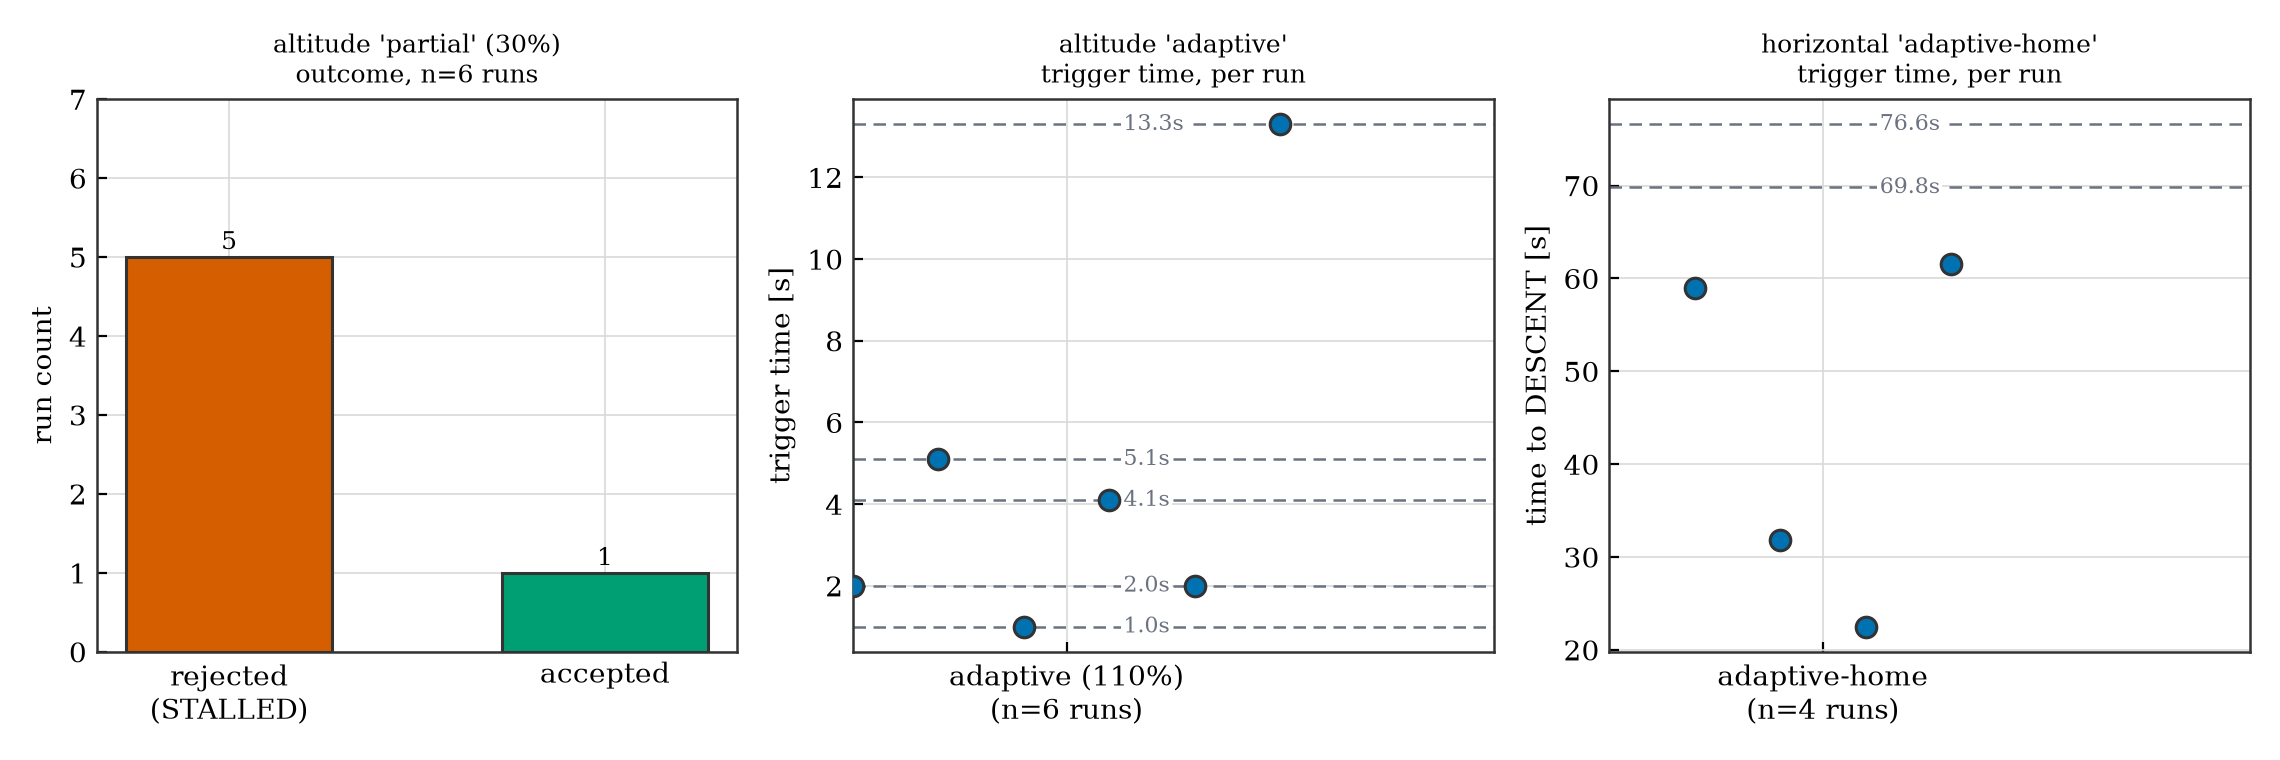
\includegraphics[width=0.7\textwidth, height=2.4in, keepaspectratio]{figures/fig3_distribution.png}
\caption{Distribution study: repeated runs of the three profiles found to be bimodal.}
\end{figure}

\vspace{2em}

\begin{figure}[H]
\centering
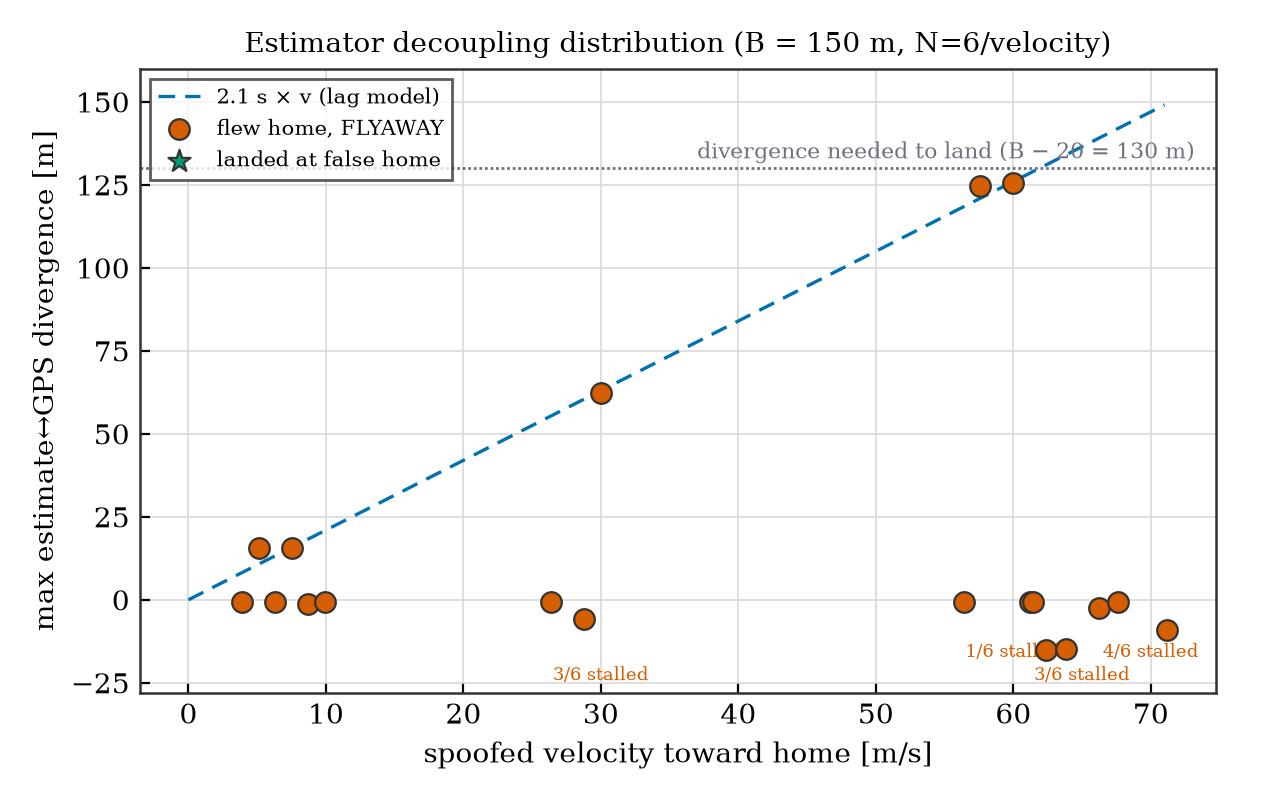
\includegraphics[width=0.8\textwidth, height=2.2in, keepaspectratio]{figures/fig4_false_home.png}
\caption{Estimator decoupling: max estimate-vs-GPS divergence vs spoofed velocity (B=150 m).}
\end{figure}

\vspace{2em}

\begin{figure}[H]
\centering
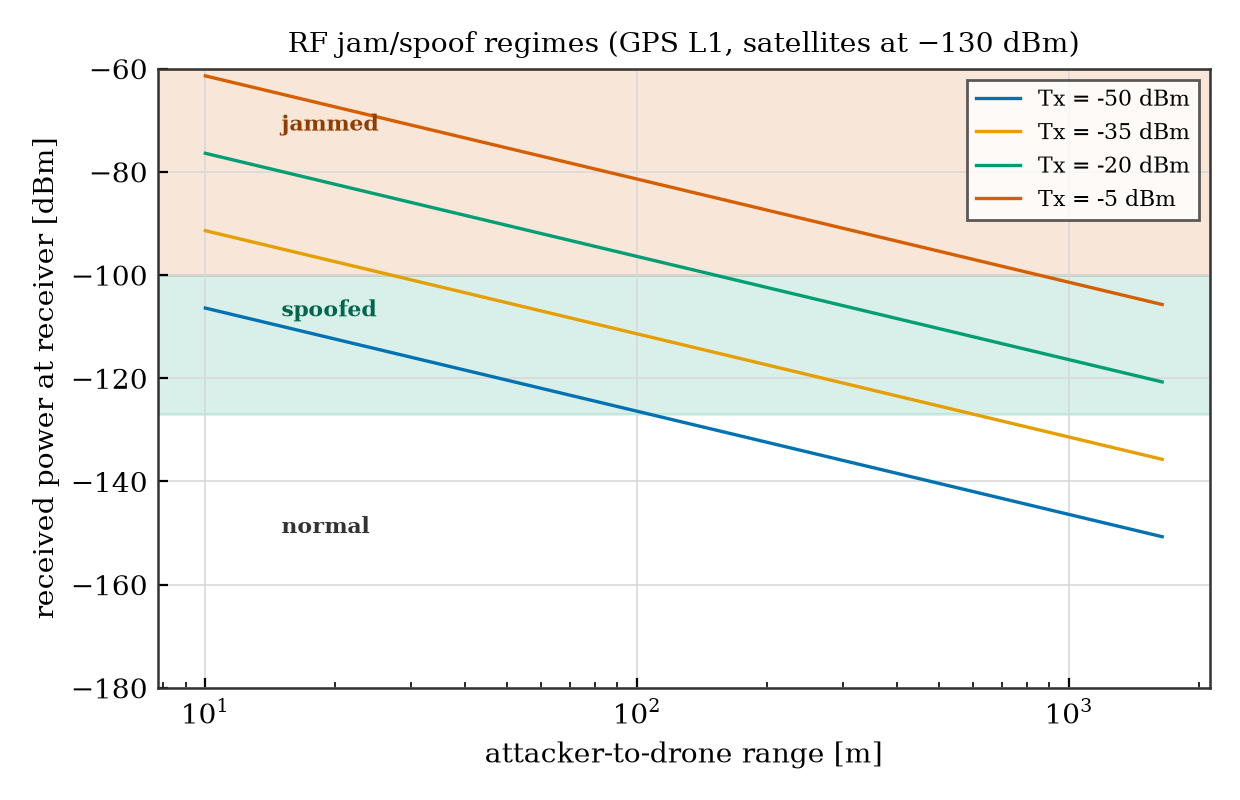
\includegraphics[width=0.8\textwidth, height=2.2in, keepaspectratio]{figures/fig5_rf_regimes.png}
\caption{RF jam/spoof regimes vs range for several transmit powers.}
\end{figure}

\vspace{2em}

\begin{figure}[H]
\centering
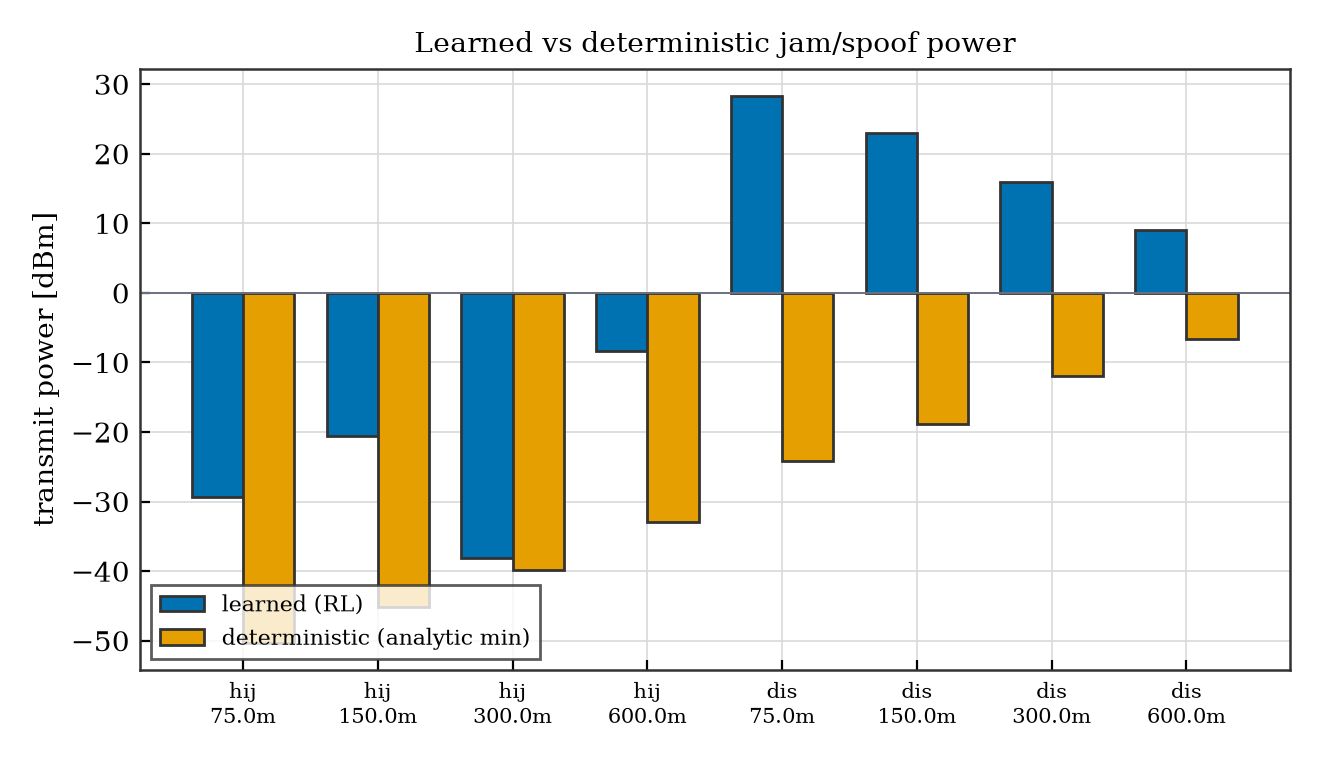
\includegraphics[width=0.8\textwidth, height=2.2in, keepaspectratio]{figures/fig6_rf_policy.png}
\caption{Learned vs deterministic jam/spoof transmit power per (goal, range).}
\end{figure}

\newpage
\section*{Appendix C: Reproducibility and Code Access}
Firmware, physics engine, attack harness, and analysis are available at:

\textbf{https://github.com/r15i/tractorbeam}

Every number and chart in this report is regenerated directly from the attack dataset by the commands below; nothing is typed into the text by hand.

The simulation was performed on an Intel Core i5-7300U (2 cores / 4 threads at 2.6 GHz) with 16 GB RAM running Linux.

\begin{table}[H]\centering\small
\caption{\textbf{Measured wall-clock cost of a full reproduction on the reference laptop.}}
\begin{tabular}{l c c}
\toprule
\textbf{Stage} & \textbf{SITL runs} & \textbf{Wall-clock} \\
\midrule
Firmware build & - & $\sim$1.5 min\\
Sanity sweeps & $\sim$24 & 13.5 min\\
False-home sweep & 31 & 40 min\\
RL training & - & 14 s\\
Integrated scenario & - & < 5 s\\
Full reproduction & $\sim$55 & $\sim$55 min \\
\bottomrule
\end{tabular}
\end{table}

\begin{quote}\small
\begin{verbatim}
# Prerequisites: git, just, uv, and a C toolchain (gcc/make).
git clone https://github.com/r15i/tractorbeam.git
cd tractorbeam

# One command runs the entire pipeline from scratch:
just all             # clean, build SITL, run every experiment, generate figures

# Or run the stages individually:
just build-sitl      # Compile Betaflight SITL (GPS Rescue sanity-check build)
just simulate        # Vertical + horizontal sanity-check sweeps
just false-home      # Estimator-decoupling / false-home landing sweep
just rf-rl           # Train the tabular soft-Q-learning (discrete SAC) agent
just scenario        # Integrated jam -> track -> spoof -> land scenario
just figures         # Render CSV data into publication figures
\end{verbatim}
\end{quote}

The environment is completely self-contained. The harness orchestrates the network sockets to the SITL binaries, verifies the attack success in real-time, and exports the measurements that generate the paper's figures.

\end{document}
